\documentclass[12pt, twoside,a4paper]{article}
\oddsidemargin = 10pt
\textwidth = 430pt

\usepackage{fullpage}	 %to make smaller margins
\usepackage{graphicx}
%\usepackage[utf8]{inputenc}
%\usepackage[T1]{fontenc}
%\usepackage{url}

\usepackage[hidelinks]{hyperref}
\usepackage{pdfpages}
\usepackage{placeins}
\usepackage{graphicx}
\usepackage[font=small,labelfont=bf]{caption}
\usepackage{subfig}

%\usepackage{subcaption}
\usepackage{enumerate}
\usepackage{amsmath}
\usepackage{listings} %for showing program code
\usepackage{bm}
\usepackage{wrapfig}
\usepackage{lipsum}
\usepackage{float}
\usepackage{titlesec}	
\usepackage{amsfonts}
\usepackage{amssymb}
\usepackage[comma,authoryear]{natbib}
\usepackage{epstopdf}


%\titlespacing*{\chapter}{0pt}{-10pt}{20pt}
%\titleformat{\chapter}[display]{\normalfont\huge\bfseries}{}{35pt}{}

\setlength{\intextsep}{0pt} %to make wrapfigures beautiful
%\setlength{\oddsidemargin}{0.5cm}
%\setlength{\evensidemargin}{-0.5cm}
\begin{document}
Given the general rendering equation
$$
L_o(x_o, \vec{\omega}_o) = L_e(x_o, \vec{\omega}_o) + L_r(x_o, \vec{\omega}_o)  
$$
$$
L_o(x_o, \vec{\omega}_o) = L_e(x_o, \vec{\omega}_o) + \int_A \int_{2 \pi} S(x_i, \vec{\omega}_i, x_o, \vec{\omega}_o) L_i(x_i, \vec{\omega}_i) (\vec{\omega}_i \cdot \vec{n}_i) d \vec{\omega}_i dA 
$$
I discretize it this way (not considering emitted radiance):


$$
L_o(x_o, \vec{\omega}_o) = \sum_{i = 0}^{N} S(x_i, \vec{\omega}_i, x_o, \vec{\omega}_o) L_i(x_i, \vec{\omega}_i) A_i 
$$
Where $A_i$ is the barycentric area (sum of vertex to the neighboring triangles to closest barycenter), and N is the number of vertices of the mesh.

The result we obtain looks correct, apart from a singularity band that happens when the refracted light direction and the normal are perpendicular, that is:

$$
 \vec{\omega}_{12}  \cdot  \vec{n}_o \approx 0
$$

In this case, the frontlit/backlit adjustment gives a value for $d_r$ close to zero, that actually causes the singularity, since 

$$
S_d \propto \frac{1}{{d_r}^3}
$$

Because of the coarse approximation used with the vertices, we are missing the points that can give us a better estimation at the point of interest. In fact, if we use a better tessellation for the mesh, we can reduce the band ideally to zero, as we can see in \ref{fig:img}. However, for the tests I was able to prepare this shrinking seems slow to converge.

\begin{figure}
\centering
\subfloat[100 vertices]{
  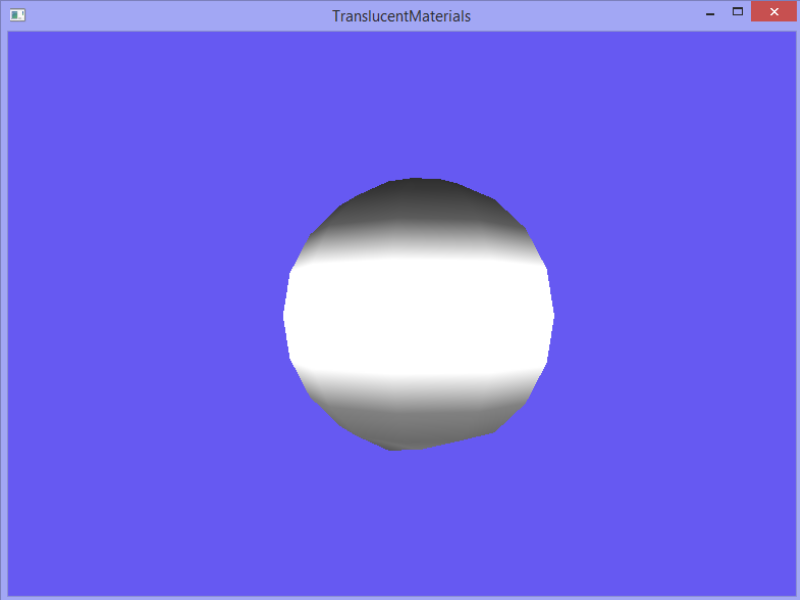
\includegraphics[width=0.3 \linewidth]{10}
  \label{fig:ss1}
}
\subfloat[400 vertices]{
  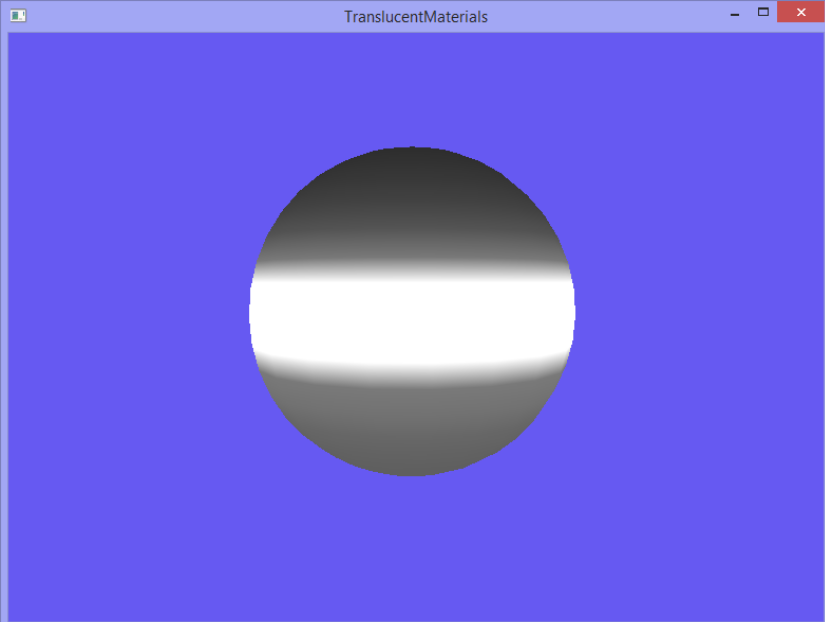
\includegraphics[width=0.3 \linewidth]{20}
  \label{fig:ss2}
} 
\subfloat[900 vertices]{
  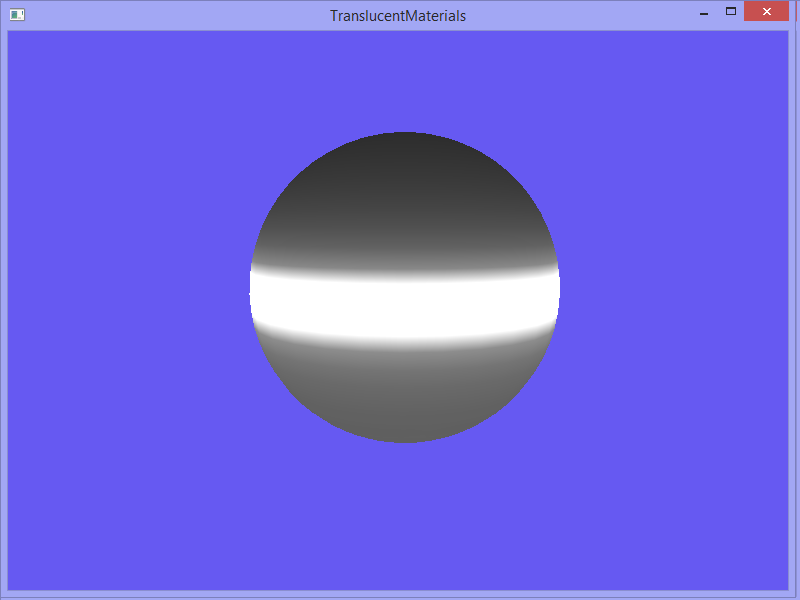
\includegraphics[width=0.3 \linewidth]{30}
  \label{fig:ss3}
} 
\\
\subfloat[1600 vertices]{
  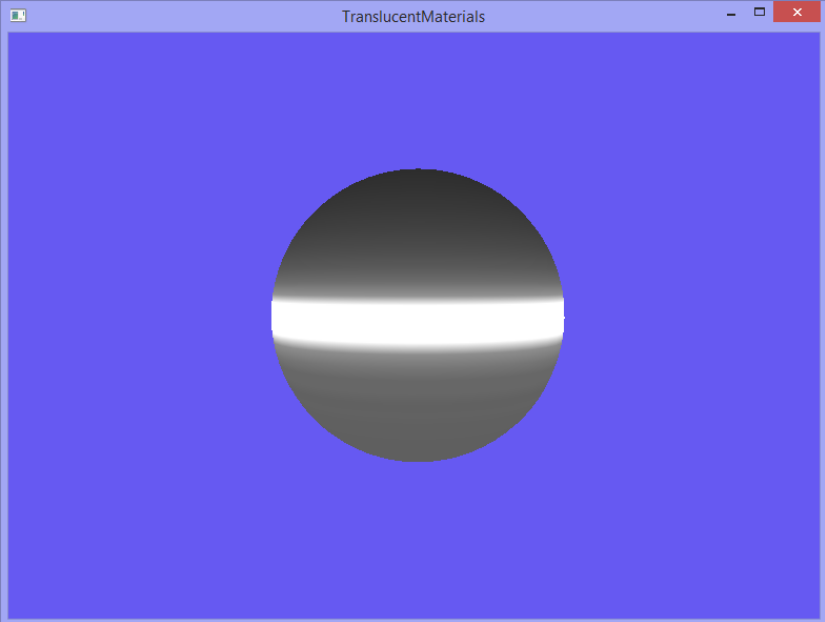
\includegraphics[width=0.3 \linewidth]{40}
  \label{fig:ss1}
}
\subfloat[2500 vertices]{
  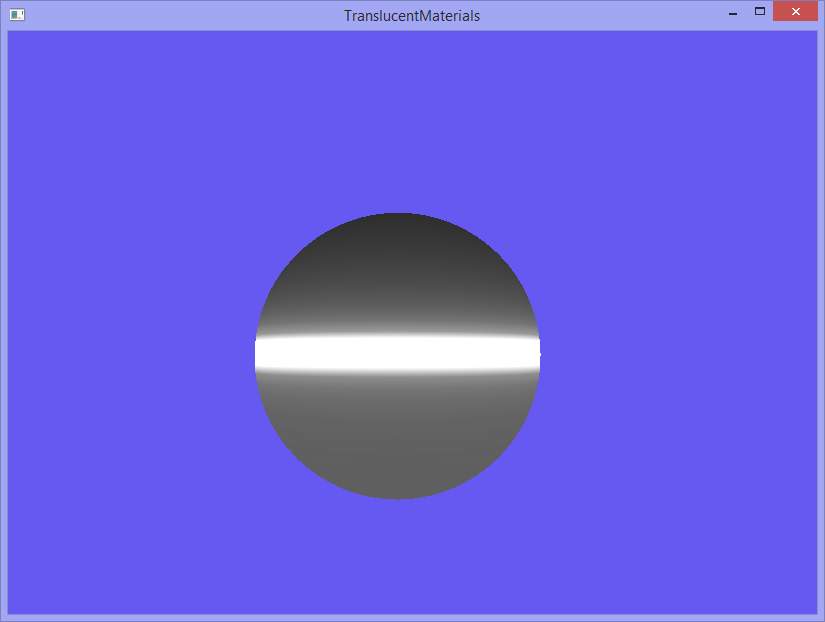
\includegraphics[width=0.3 \linewidth]{50}
  \label{fig:ss2}
} 
%\subfloat[3600 vertices]{
%  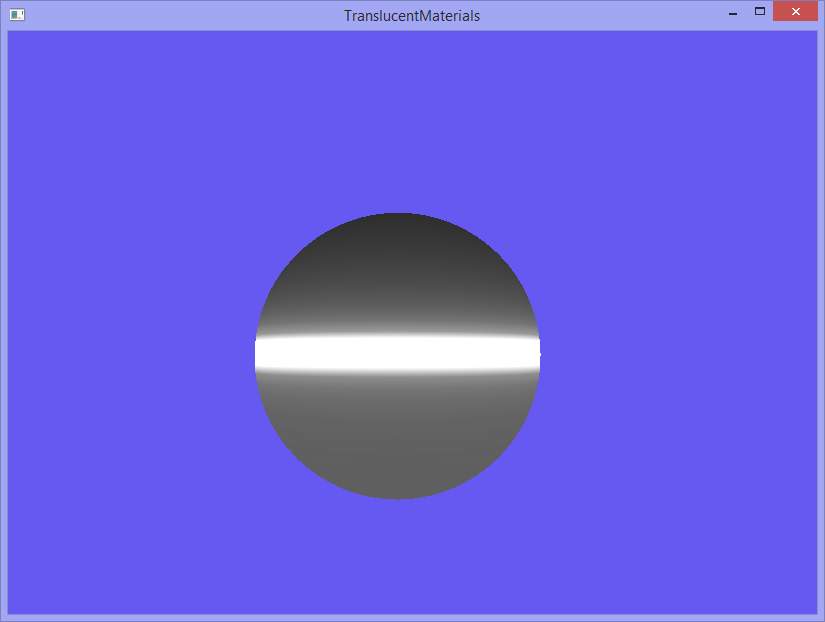
\includegraphics[width=0.3 \linewidth]{60}
%  \label{fig:ss3}
%} 

\caption{Shrinking band for growing number of vertices.}
\label{fig:img}
\end{figure}

\begin{figure}[here]
\centering
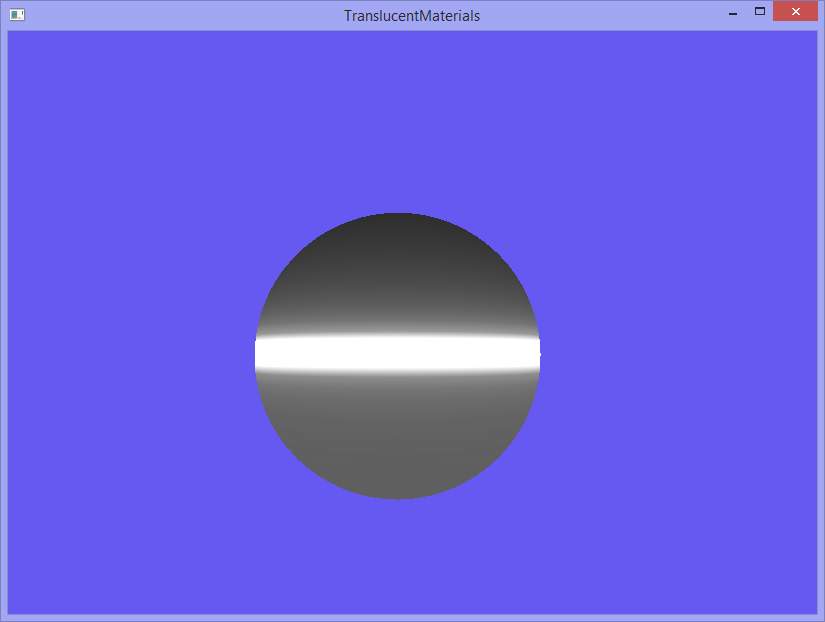
\includegraphics[width=0.8\textwidth]{50}
\caption{Full image.}
\label{fig:ssdiagram}
\end{figure}



\begin{figure}
\centering
\subfloat[0.05]{
  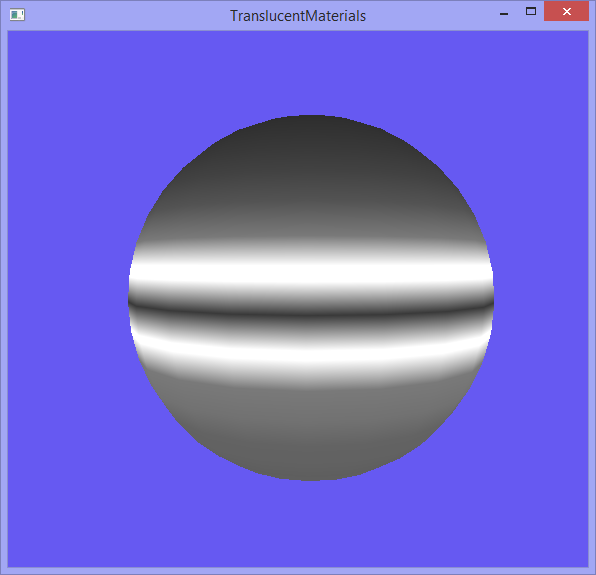
\includegraphics[width=0.45 \linewidth]{005}
  \label{fig:ss1}
}
\\
\subfloat[0.2]{
  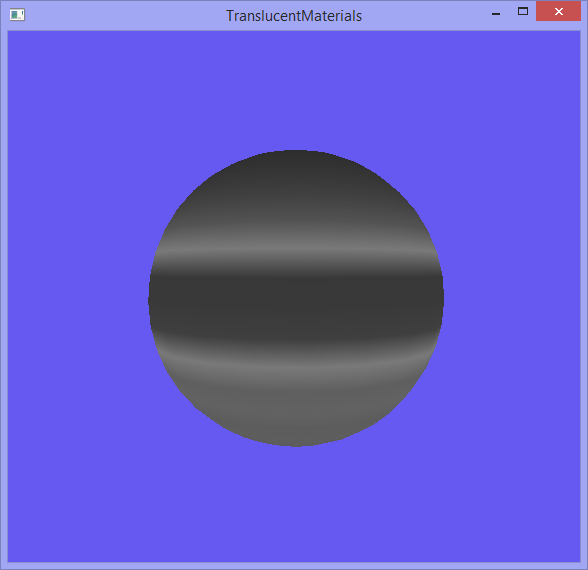
\includegraphics[width=0.45 \linewidth]{02}
  \label{fig:ss2}
} 
\\
\subfloat[0.4]{
  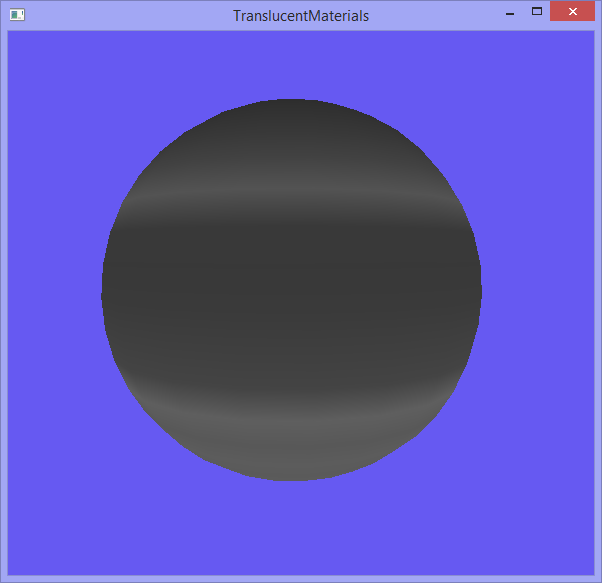
\includegraphics[width=0.45 \linewidth]{04}
  \label{fig:ss3}
} 


\caption{Different Thresolds for $\mu_0$.}
\label{fig:img2}
\end{figure}
\end{document}
